\documentclass{article}

% Language setting
% Replace `english' with e.g. `spanish' to change the document language
\usepackage[english]{babel}

% Set page size and margins
% Replace `letterpaper' with `a4paper' for UK/EU standard size
\usepackage[letterpaper,top=2cm,bottom=2cm,left=3cm,right=3cm,marginparwidth=1.75cm]{geometry}

% Useful packages
\usepackage{amsmath}
\usepackage{amssymb}
\usepackage{graphicx}
\usepackage[colorlinks=true, allcolors=blue]{hyperref}

\begin{document}

\section{CERN, the LHC, and the CMS Experiment}

\subsection{CERN and the Large Hadron Collider}
% [CITE] https://cds.cern.ch/record/782076
The European Council for Nuclear Research (in French \textit{Conseil Europ\'{e}en pour la Recherche Nucl\'{e}aire}), also known as CERN, is the site of an accelerator complex hosting the Large Hadron Collider (LHC). The LHC consists of a 27-kilometer ring of superconducting magnets with accelerating structures to boost the energy of particles, which collide at a center-of-mass energy of up to 14 TeV. The beams inside the LHC are made to collide at four locations around the accelerator ring, at the locations of four particle detectors: ATLAS, CMS, ALICE, and LHCb.

The number of events generated per second at the LHC collisions is given by $N_{event} = \mathcal{L} \sigma_{event}$, where $\sigma_{event}$ is the cross-section for the event under study, and $\mathcal{L}$ the machine luminosity. The machine luminosity depends only on the beam parameters, and can be written for a Gaussian beam distribution as:

\begin{equation}
    \mathcal{L} = \frac{N_b^2 n_b f_{rev} \gamma_r}{4\pi \epsilon_n \beta^*} F
\end{equation}
where $N_b$ is the number of particles per bunch, $n_b$ the number of bunches per beam, $f_{rev}$ the revolution frequency, $\gamma_r$ the relativistic gamma factor, $\epsilon_n$ the normalized transverse beam emittance, $\beta^*$ the beta function at the collision point, and $F$ the geometric luminosity reduction factor due to the crossing angle at the interaction points. Luminosity is measured in units of cm$^{-2}$ s$^{-1}$. Thus the exploration of rare events in the LHC collisions requires both high beam energies and high beam intensities.

\subsection{The CMS Detector}
% cite https://iopscience.iop.org/article/10.1088/1748-0221/3/08/S08004/pdf
The Compact Muon Solenoid (CMS) experiment was conceived to study proton-proton and lead-lead collisions at a center-of-mass energy of 14 TeV (5.5 TeV nucleon-nucleon) and at luminosities up to $10^{34}$ cm$^{-2}$ s$^{-1}$ ($10^{27}$ cm$^{-2}$ s$^{-1}$). At the center of the CMS detector, a high-magnetic-field superconducting solenoid surrounds a silicon pixel and strip tracker, a lead-tungstate scintillating-crystals electromagnetic calorimeter (ECAL), and a brass-scintillator sampling hadron calorimeter (HCAL). The iron yoke of the flux-return houses four stations of gas-ionization chamber muon detectors. The collision data is recorded with the use of the Level-1 (L1) trigger, high-level trigger (HLT), and data acquisition systems ensuring high efficiency in selecting physics events of interest. A detailed description of the CMS detector can be found in [CITE].

% not super clean citation: Tracker TDR https://cds.cern.ch/record/2272264/files/CMS-TDR-014.pdf
CMS uses a right-handed coordinate system [CITE]. The origin is centered at the nominal collision point inside the experiment. The $x$ axis points towards the center of the LHC, and the $y$ axis points vertically upwards. The $z$ axis points along the beam direction. The azimuthal angle, $\phi$, is measured from the $x$ axis in the $x$-$y$ plane, and the radial coordinate in this plane is denoted by $r$. The polar angle, $\theta$, is measured from the $z$ axis. The pseudorapidity, $\eta$, is defined as $\eta = -\ln \tan(\theta/2)$. The momentum and energy transverse to the beam direction, denoted by $p_{T}$ and $E_{T}$ respectively, are computed from the $x$ and $y$ components. The momentum imbalance in the transverse plane is called the missing transverse momentum, and its magnitude is denoted by $E_{T}^{\text{miss}}$.

\subsection{Sub-detectors of CMS}
This section details the sub-detectors of CMS that operate to identify and precisely measure muons, electrons, photons, and jets over a large energy range. 

\subsubsection{Inner tracking system}
% CITE: Original Tracker TDR https://cds.cern.ch/record/368412/files/Tracker_TDR.pdf
% CITE: Phase-1 Tracker TDR: https://cds.cern.ch/record/1481838 
% CITE: Phase-2 https://cds.cern.ch/record/2272264/files/CMS-TDR-014.pdf
The CMS Tracker perform robust tracking and detailed vertex reconstruction in the 4 T magnetic field of the superconducting solenoidal magnet. The active envelope of the CMS Tracker extends to a radius of 115 cm, over a length of approximately 270 cm on each side of the interaction point [CITE] %original tracker TDR. 
Charged particles in the region $|\eta| \lesssim 1.6$ benefit from the full momentum measurement precision. In this region, a charged particle with $p_T$ of 1000 GeV has a sagitta of $\sim 195$ $\mu$m. The Tracker acceptance extends further to $|\eta| = 2.5$, with a reduced radial lever arm of approximately 50 cm.

The high magnetic field of CMS causes low $p_{T}$ charged particles to travel in helical trajectories with small radii. The majority of events contain particles with a steeply falling $p_{T}$ spectrum, resulting in a track density which rapidly decreases at higher radii. 

\begin{figure}[ht]
    \centering
    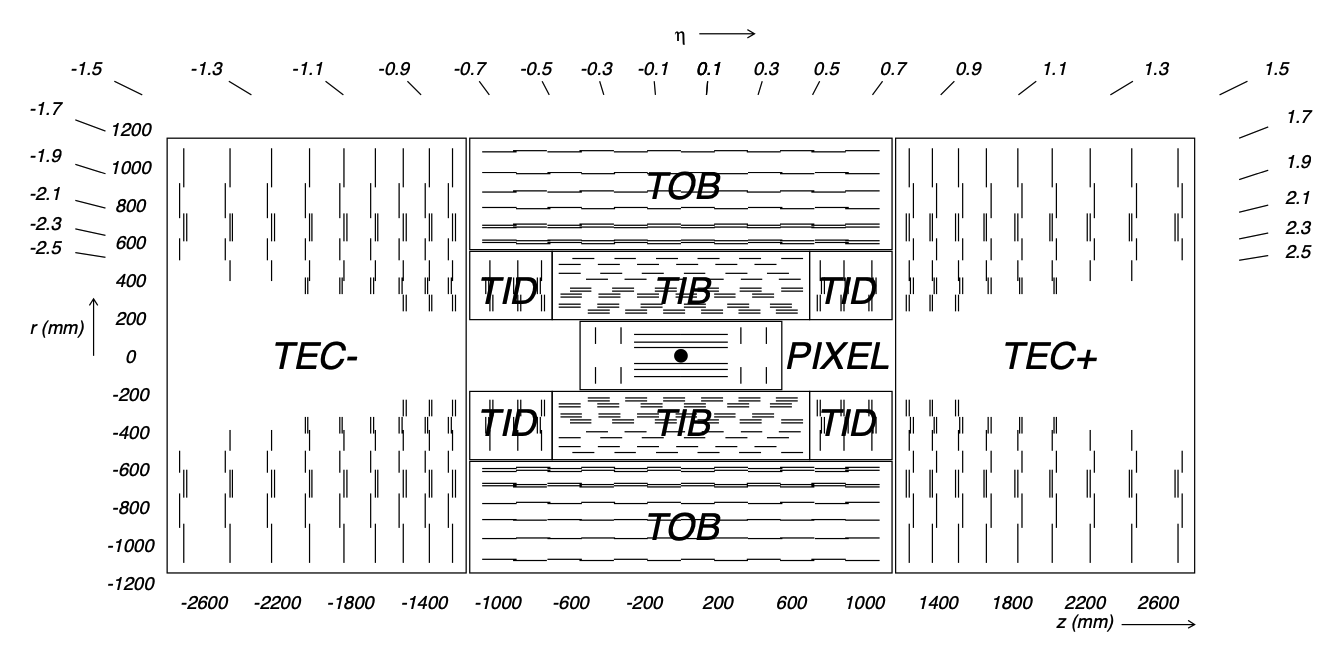
\includegraphics[width=11cm]{figures/phase-1-tdr-tracker-schematic.png}
    \caption{Cross section of the current Phase-1 CMS tracker from [CITE] https://cds.cern.ch/record/1481838/files/CMS-TDR-011.pdf, showing the nomenclature of different sections. Each line represents a detector module. Double lines indicate back-to-back modules which deliver stereo hits in the strip tracker.}
    \label{fig:phase-1-tdr-tracker-schematic}
\end{figure}


A schematic view of the current Phase-1 CMS tracker, including the pixel detector, is shown in Fig. \ref{fig:phase-1-tdr-tracker-schematic}. The Phase-1 pixel detector consists of three barrel layers (BPIX) at radii of 4.4 cm, 7.3 cm, and 10.2 cm, and two forward/backward disks (FPIX) at longitudinal positions of $\pm$ 34.5 cm and $\pm$ 46.5 cm, and extending in radius from about 6 cm to 15 cm. These pixelated detectors produce 3D measurements along the paths of charged particles with single hit resolutions between 10-20 $\mu$m. 

% here cite https://iopscience.iop.org/article/10.1088/1748-0221/3/08/S08004/pdf
After the pixel and on their way out of the tracker, particles pass through the silicon strip tracker which reaches out to a radius of 130 cm (Fig. \ref{fig:phase-1-tdr-tracker-schematic}). The sensor elements in the strip tracker are single-sided $p$-on-$n$ type silicon micro-strip sensors [CITE 2008 CMS]. The silicon strip detector consists of four inner barrel (TIB) layers assembled in shells, with two inner endcaps (TID), each composed of three small discs. The outer barrel (TOB) consists of six concentric layers. Two endcaps (TEC) close off the tracker on either end. 


\subsubsection{ECAL} 



\subsubsection{HCAL}

\subsubsection{Muon detectors}

\subsection{The Level-1 Trigger}

\subsection{The Phase-2 Upgrade of the CMS detector}
% Tracker Phase-2: https://cds.cern.ch/record/2272264/files/CMS-TDR-014.pdf

\end{document}